

%% Based on a TeXnicCenter-Template by Tino Weinkauf.
%%%%%%%%%%%%%%%%%%%%%%%%%%%%%%%%%%%%%%%%%%%%%%%%%%%%%%%%%%%%%

%%%%%%%%%%%%%%%%%%%%%%%%%%%%%%%%%%%%%%%%%%%%%%%%%%%%%%%%%%%%%
%% HEADER
%%%%%%%%%%%%%%%%%%%%%%%%%%%%%%%%%%%%%%%%%%%%%%%%%%%%%%%%%%%%%
\documentclass[a4paper,twoside,10pt]{report}
% Alternative Options:
%	Paper Size: a4paper / a5paper / b5paper / letterpaper / legalpaper / executivepaper
% Duplex: oneside / twoside
% Base Font Size: 10pt / 11pt / 12pt


%% Language %%%%%%%%%%%%%%%%%%%%%%%%%%%%%%%%%%%%%%%%%%%%%%%%%
\usepackage[T1]{fontenc}

\usepackage{lmodern} %Type1-font for non-english texts and characters


%% Packages for Graphics & Figures %%%%%%%%%%%%%%%%%%%%%%%%%%
\usepackage{graphicx} %%For loading graphic files
%\usepackage{subfig} %%Subfigures inside a figure
%\usepackage{pst-all} %%PSTricks - not useable with pdfLaTeX

%% Please note:
%% Images can be included using \includegraphics{Dateiname}
%% resp. using the dialog in the Insert menu.
%% 
%% The mode "LaTeX => PDF" allows the following formats:
%%   .jpg  .png  .pdf  .mps
%% 
%% The modes "LaTeX => DVI", "LaTeX => PS" und "LaTeX => PS => PDF"
%% allow the following formats:
%%   .eps  .ps  .bmp  .pict  .pntg


%% Math Packages %%%%%%%%%%%%%%%%%%%%%%%%%%%%%%%%%%%%%%%%%%%%
\usepackage{amsmath}
\usepackage{amsthm}
\usepackage{amsfonts}
\usepackage{lingmacros}
\usepackage{tree-dvips}
\usepackage[utf8]{inputenc}
\usepackage[spanish]{babel}
\usepackage{graphicx}
\usepackage{hyperref}

%% Line Spacing %%%%%%%%%%%%%%%%%%%%%%%%%%%%%%%%%%%%%%%%%%%%%
%\usepackage{setspace}
%\singlespacing        %% 1-spacing (default)
%\onehalfspacing       %% 1,5-spacing
%\doublespacing        %% 2-spacing


%% Other Packages %%%%%%%%%%%%%%%%%%%%%%%%%%%%%%%%%%%%%%%%%%%
%\usepackage{a4wide} %%Smaller margins = more text per page.
%\usepackage{fancyhdr} %%Fancy headings
%\usepackage{longtable} %%For tables, that exceed one page


%%%%%%%%%%%%%%%%%%%%%%%%%%%%%%%%%%%%%%%%%%%%%%%%%%%%%%%%%%%%%
%% Remarks
%%%%%%%%%%%%%%%%%%%%%%%%%%%%%%%%%%%%%%%%%%%%%%%%%%%%%%%%%%%%%
%
% TODO:
% 1. Edit the used packages and their options (see above).
% 2. If you want, add a BibTeX-File to the project
%    (e.g., 'literature.bib').
% 3. Happy TeXing!
%
%%%%%%%%%%%%%%%%%%%%%%%%%%%%%%%%%%%%%%%%%%%%%%%%%%%%%%%%%%%%%

%%%%%%%%%%%%%%%%%%%%%%%%%%%%%%%%%%%%%%%%%%%%%%%%%%%%%%%%%%%%%
%% Options / Modifications
%%%%%%%%%%%%%%%%%%%%%%%%%%%%%%%%%%%%%%%%%%%%%%%%%%%%%%%%%%%%%

%\input{options} %You need a file 'options.tex' for this
%% ==> TeXnicCenter supplies some possible option files
%% ==> with its templates (File | New from Template...).



%%%%%%%%%%%%%%%%%%%%%%%%%%%%%%%%%%%%%%%%%%%%%%%%%%%%%%%%%%%%%
%% DOCUMENT
%%%%%%%%%%%%%%%%%%%%%%%%%%%%%%%%%%%%%%%%%%%%%%%%%%%%%%%%%%%%%
\begin{document}

\pagestyle{empty} %No headings for the first pages.


%% Title Page %%%%%%%%%%%%%%%%%%%%%%%%%%%%%%%%%%%%%%%%%%%%%%%
%% ==> Write your text here or include other files.

%% The simple version:
\title{%
  Propuesta de Diseño de Aplicación Funcional\\
  \large Registro y Mantenimiento de Extinctores \\
    Team Brije}

\author{
  Shika Moriyama
  \and
  Amaury Flores
	\and
  Carol Torres
	\and
  Wilbert Arcila
}
%\date{} %%If commented, the current date is used.
\maketitle

%% The nice version:
%\input{titlepage} %%You need a file 'titlepage.tex' for this.
%% ==> TeXnicCenter supplies a possible titlepage file
%% ==> with its templates (File | New from Template...).


%% Inhaltsverzeichnis %%%%%%%%%%%%%%%%%%%%%%%%%%%%%%%%%%%%%%%
\tableofcontents %Table of contents
\cleardoublepage %The first chapter should start on an odd page.

\chapter{Propuesta uno}

\section{Un Pequeño Resumen}

\par De forma breve, la aplicación que se piensa realizar es un generador y lector de códigos QR el cual almacene información de Extintores como su ubicación, fecha de mantenimiento y seguridad, entre otros. Para esto, se buscará crear una app que tenga tres principales elementos.

\section{Requerimientos Funcionales}

\par Estos son los requerimientos funcionales que deben de ser abarcados:
\begin{itemize}
	\item Poder borrar TODOS los extintores de golpe.
	\item Poder leer estos códigos generados.
	\item Poder agregar, editar y eliminar extintores de una lista
	\item Poder agregar información a cada extintor en la lista
\end{itemize}

\section{Requerimientos No Funcionales}

\par Estos son los requerimientos no funcionales que deben de ser abarcados:
\begin{itemize}
	\item Uso y gestión de base de datos 
	\item Transformar IDs de diferentes elementos de la base de datos a códigos. 
	\item Generar listas dinámicas según lo necesitado por el usuario
	\item Generación iterativa de cada elemento para la optimización de elementos. 
	\item Optimización de archivos para consumir la menor cantidad de espacio en el almacenamiento del sistema. 
	\item Creado en Android Studio
\end{itemize}

\section{Casos}

\begin{figure}[htbp]
	\centering
		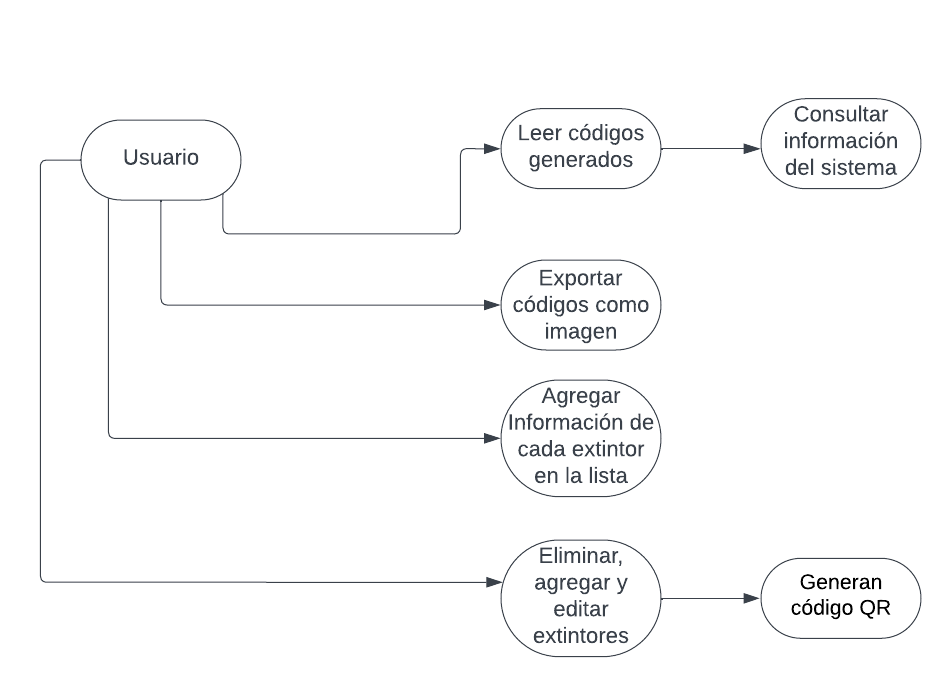
\includegraphics[width=0.70\textwidth]{Gaming1.png}
	\label{fig:Gaming1}
\end{figure}

\begin{figure}[htbp]
	\centering
		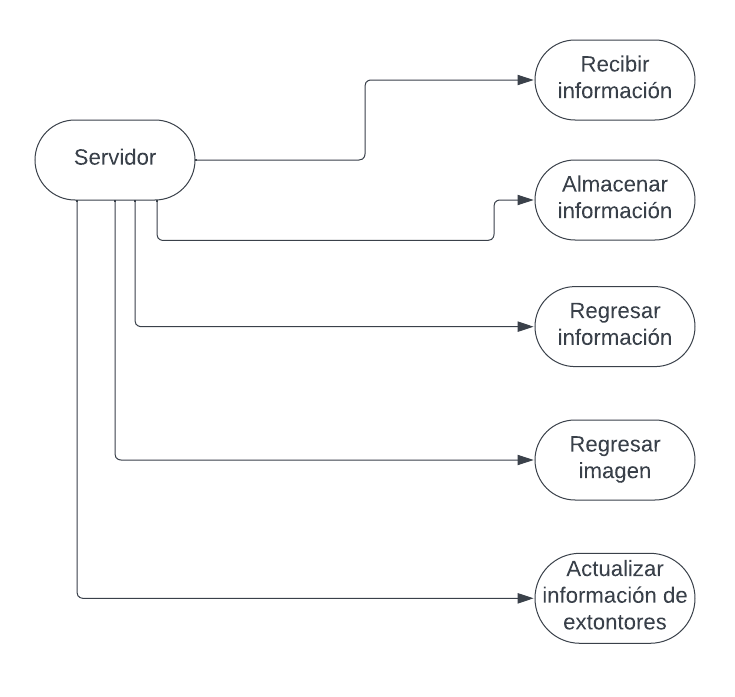
\includegraphics[width=0.70\textwidth]{Gmaing2.png}
	\label{fig:Gmaing2}
\end{figure}



\newpage 

\chapter{Segunda Propuesta}

\section{Una segunda opción}

\par Como le llegamos a comentar en clase, también teníamos otra idea, la cual también se intentará efectuar, pero lo tomaremos como un reto extra, enfocándonos en el administrador de extintores primero. La segunda opción sería una calculadora de fusiones de el juego Persona 5, la cual estaría estilizada en la estética del juego mismo.

\section{Requerimientos funcionales}

\par Estos son los requerimientos funcionales que deben de ser abarcados:

\begin{itemize}
	\item Accesar a unas de las Personas del juego
	\item Meterse a cada Persona individual, poder ver sus Stats
	\item Ver las habilidades de cada Persona, y sus ventajas de tipo
    \item Igor Bailando Cumbiab
\end{itemize}

\section{Requerimientos no funcionales}

\par Estos son los requerimientos no funcionales que deben de ser abarcados:

\begin{itemize}
	\item Será creado en UNITY
	\item Accesar a una base estatica de datos
	\item Iterar sobre una misma página
\end{itemize}

\newpage

\section{Casos}

\begin{figure}[htbp]
	\centering
		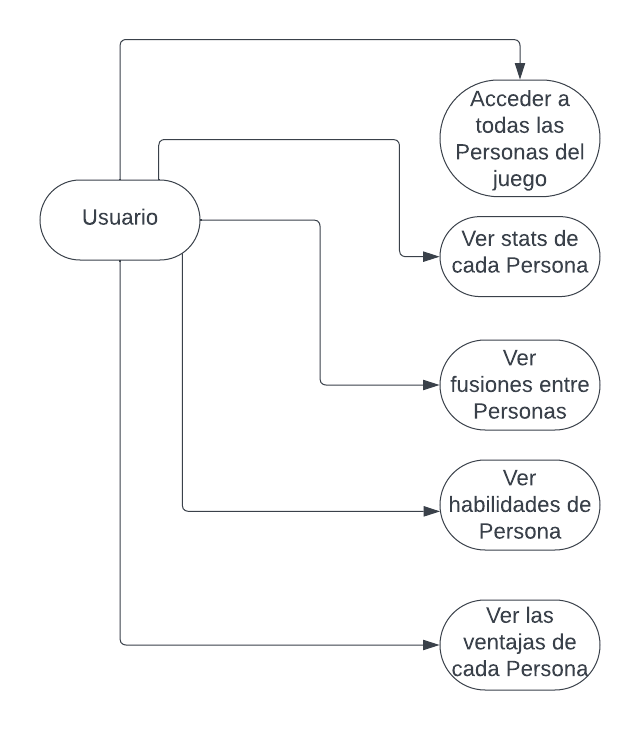
\includegraphics[width=1.00\textwidth]{Personacasos.png}
	\label{fig:Personacasos}
\end{figure}

\chapter{Diagramas}

\par Aqui vamos a poner los diagramas que hemos hecho para ambos juegos

\section{Diagrama de componentes}

		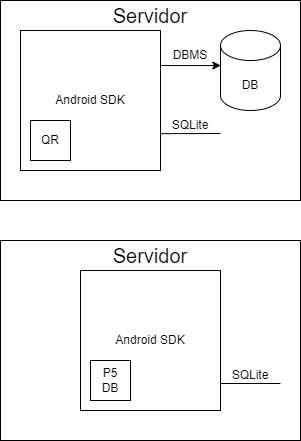
\includegraphics[width=0.50\textwidth]{APPExtntor.png}


\section{Diagrama de Entidad Relacion}

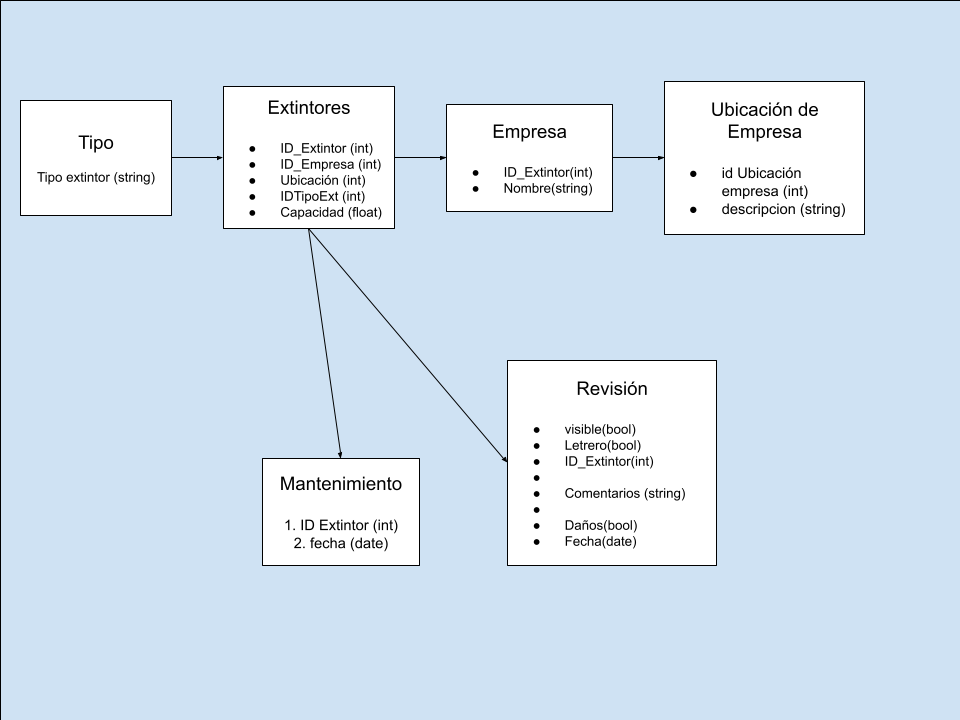
\includegraphics[width=1.0\textwidth]{Gaming.png}


\section{Diagrama de clases}


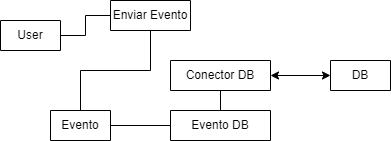
\includegraphics[width=1.0\textwidth]{ClasesExtintor.png}


\section{Diagrama de secuencia}


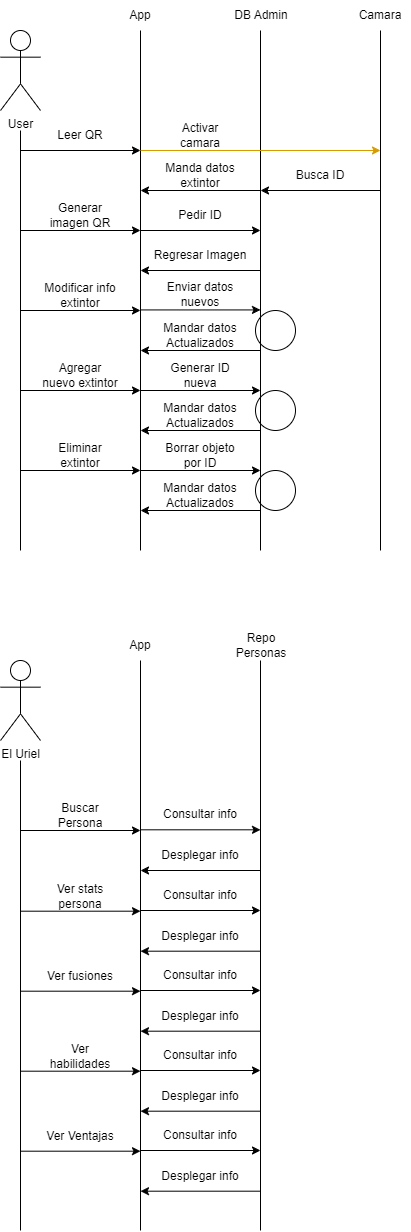
\includegraphics[width=0.50\textwidth]{Sequencia.png}


\section{Diagramas de flujo}


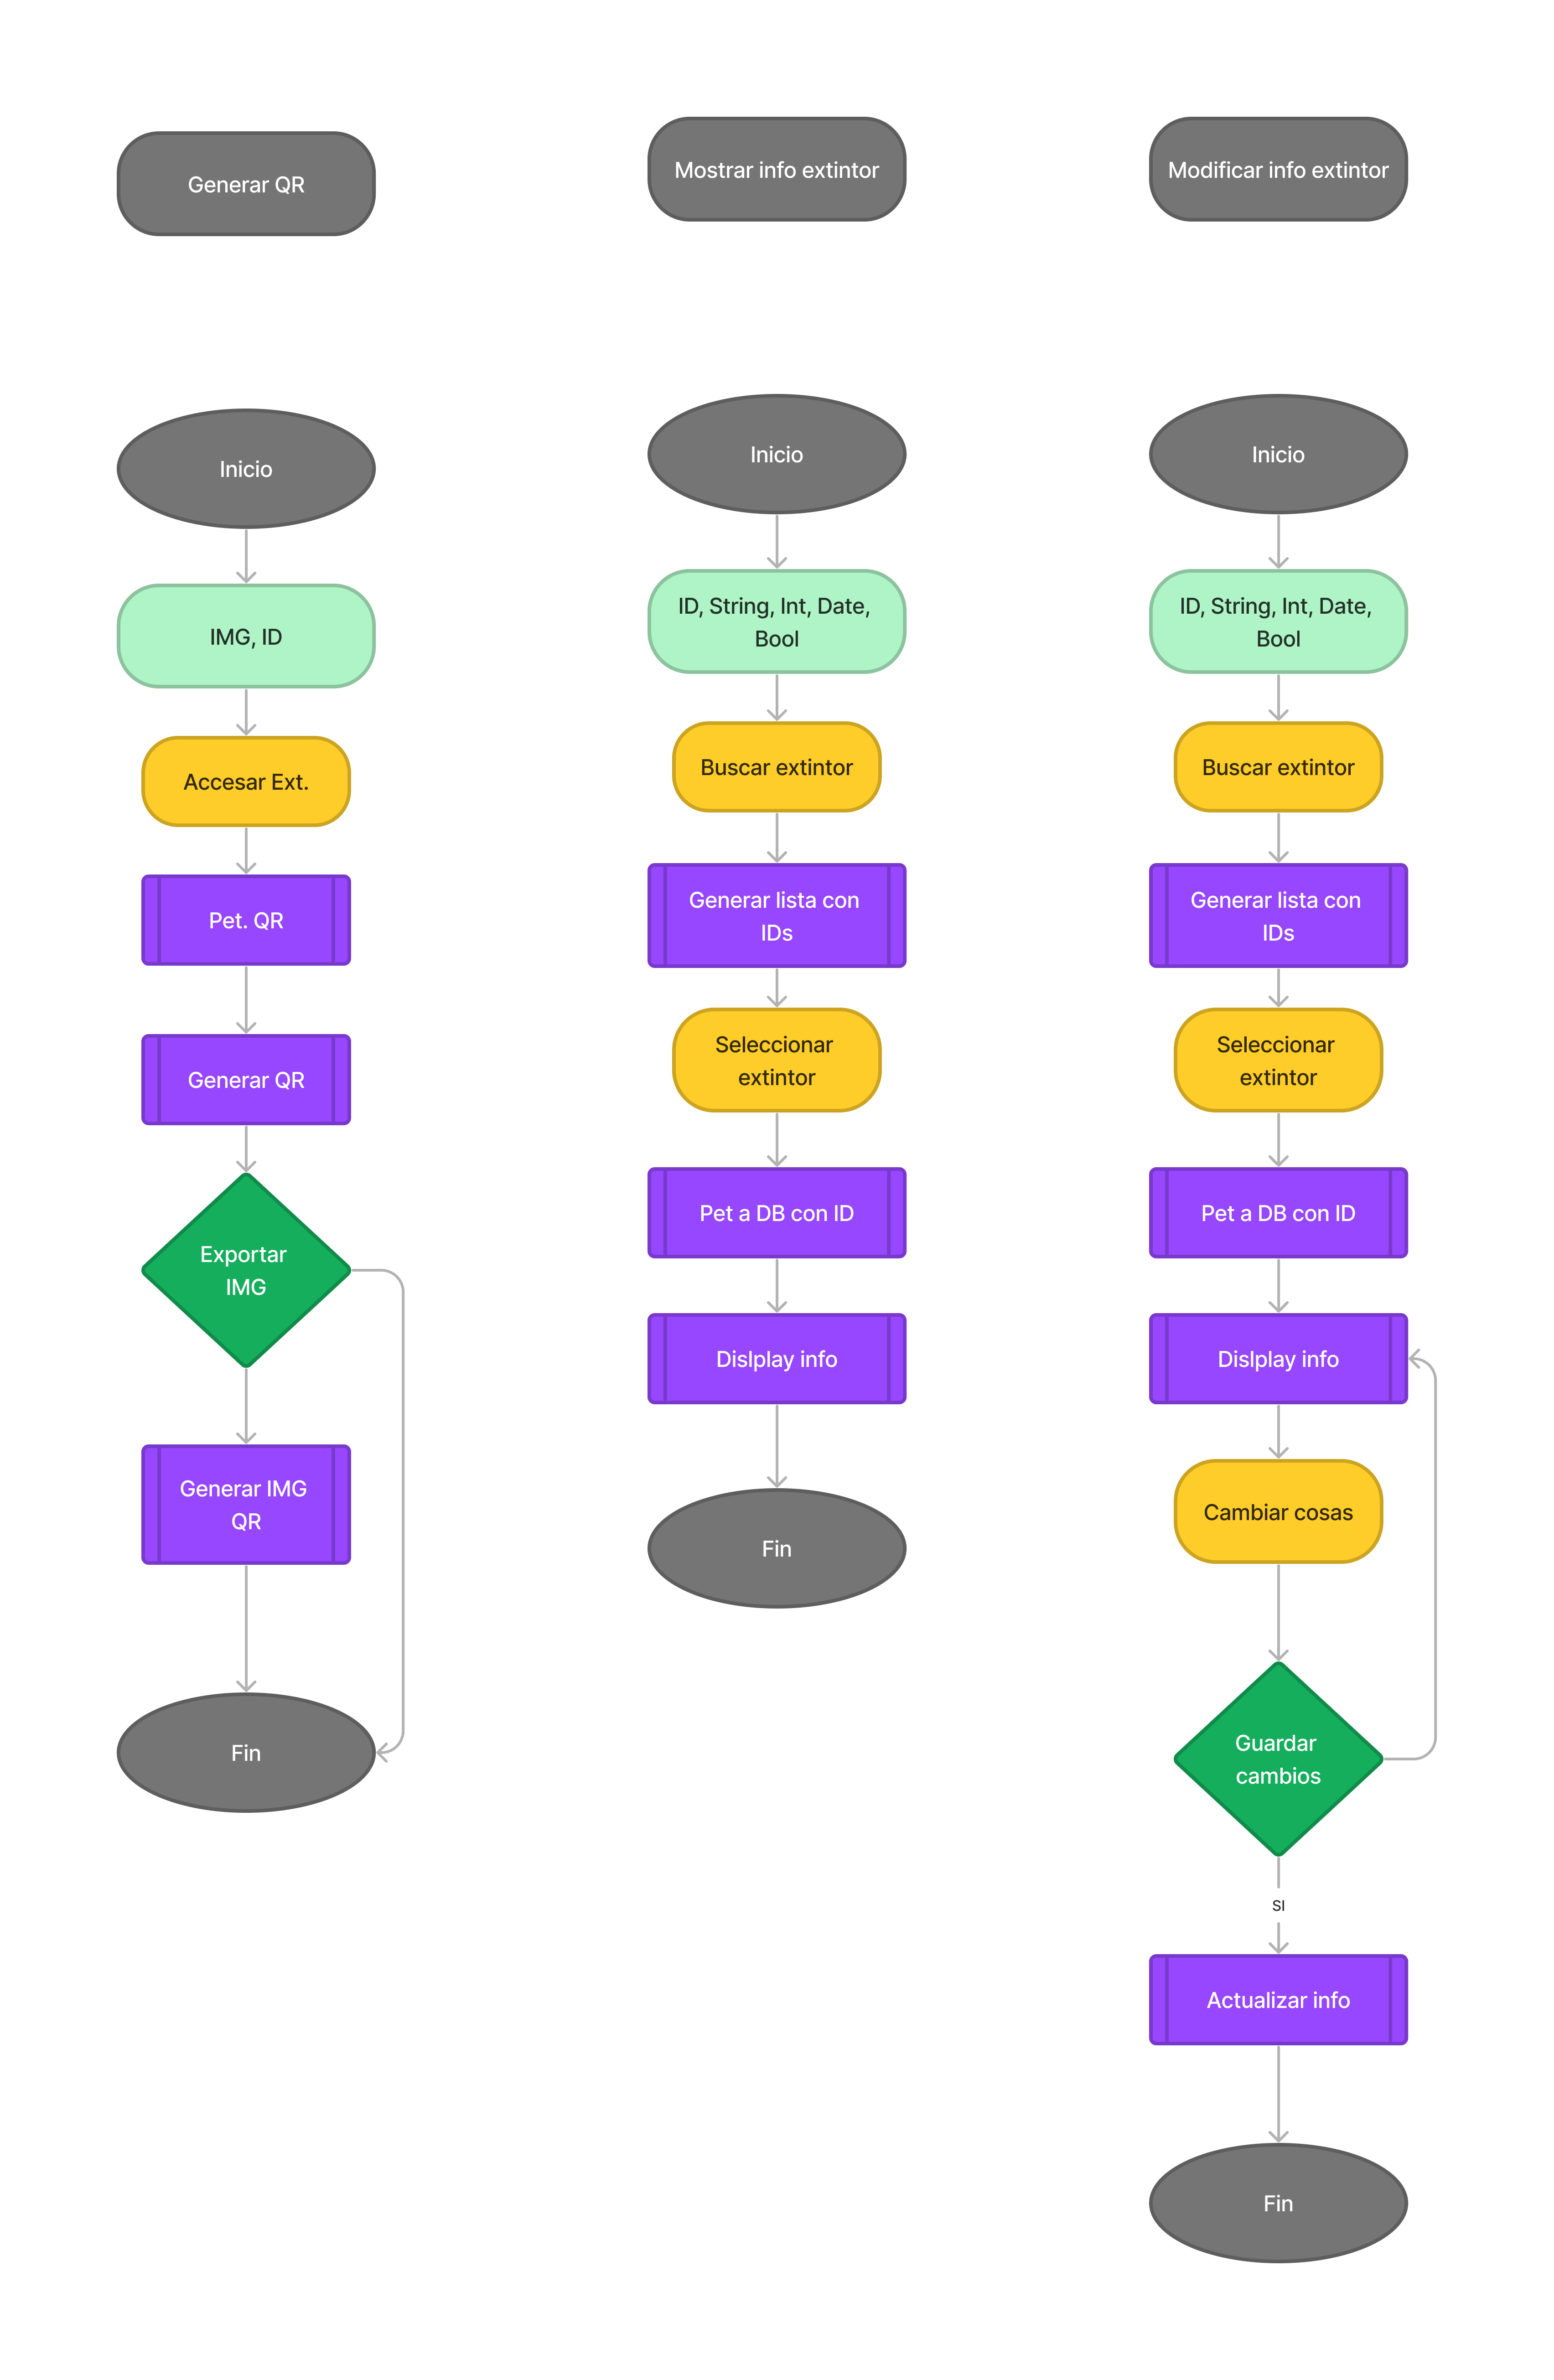
\includegraphics[width=1.0\textwidth]{GamingDiagrama1.png}

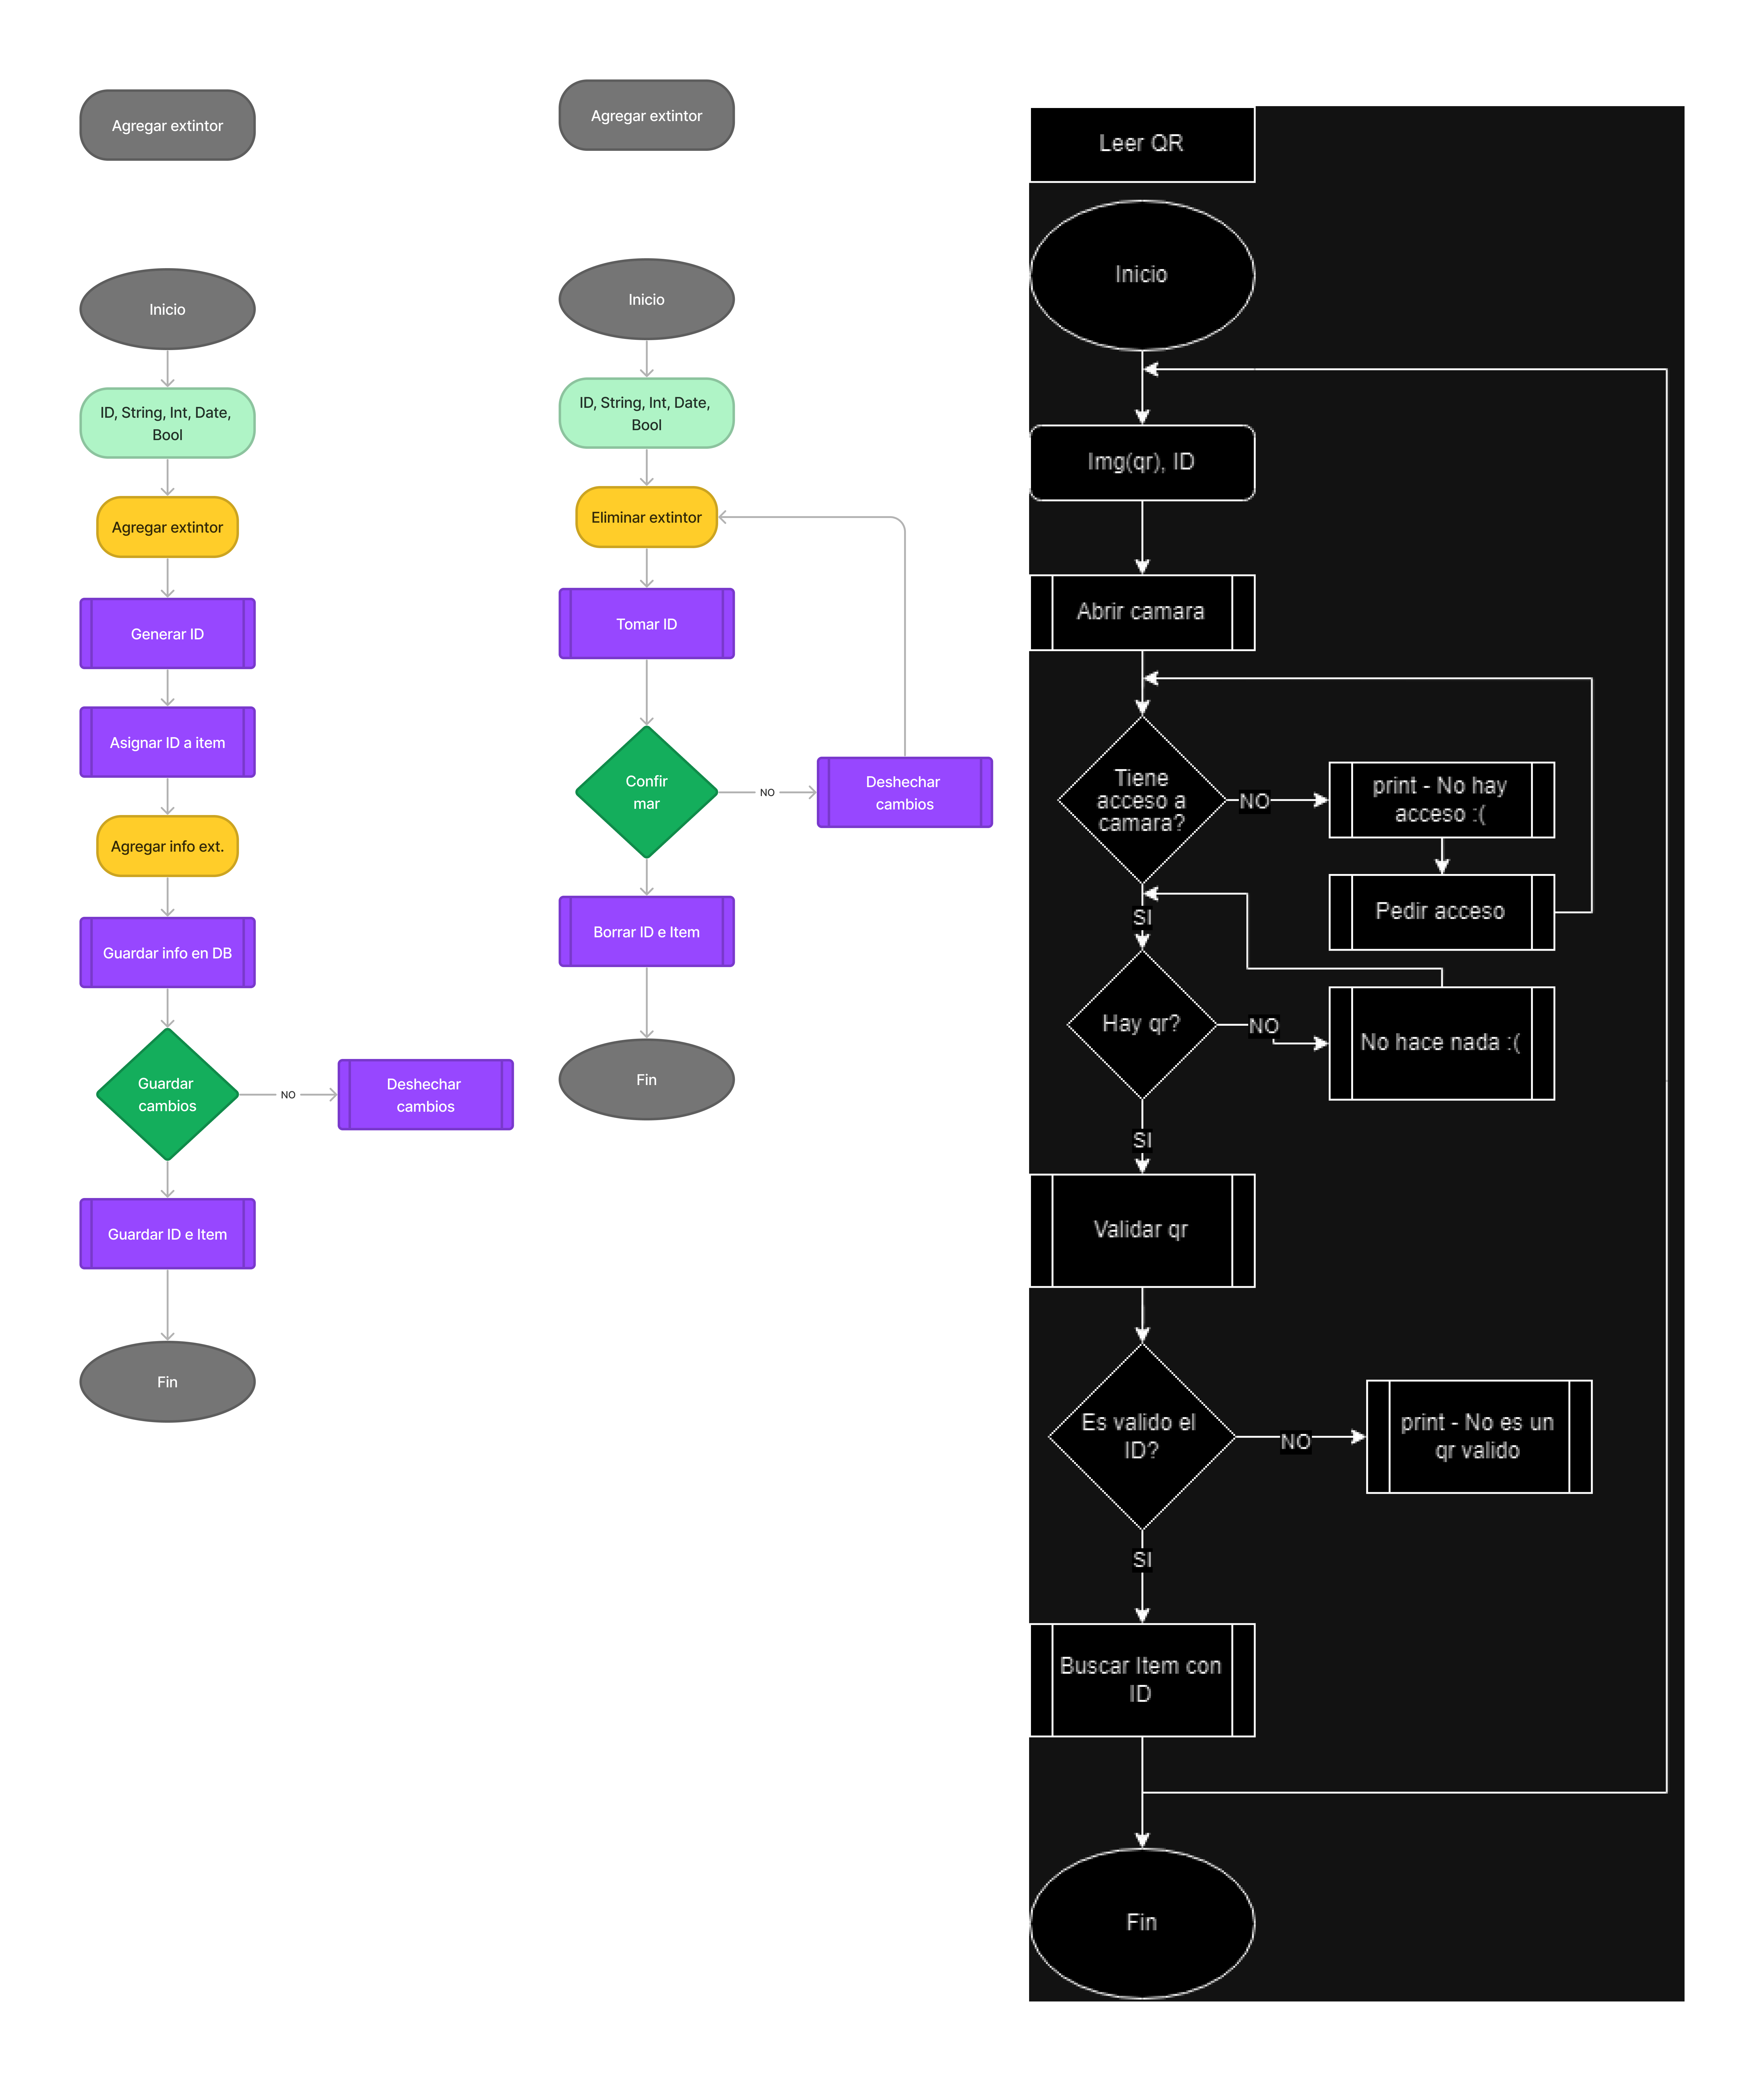
\includegraphics[width=1.0\textwidth]{GamingDiagrama2.png}

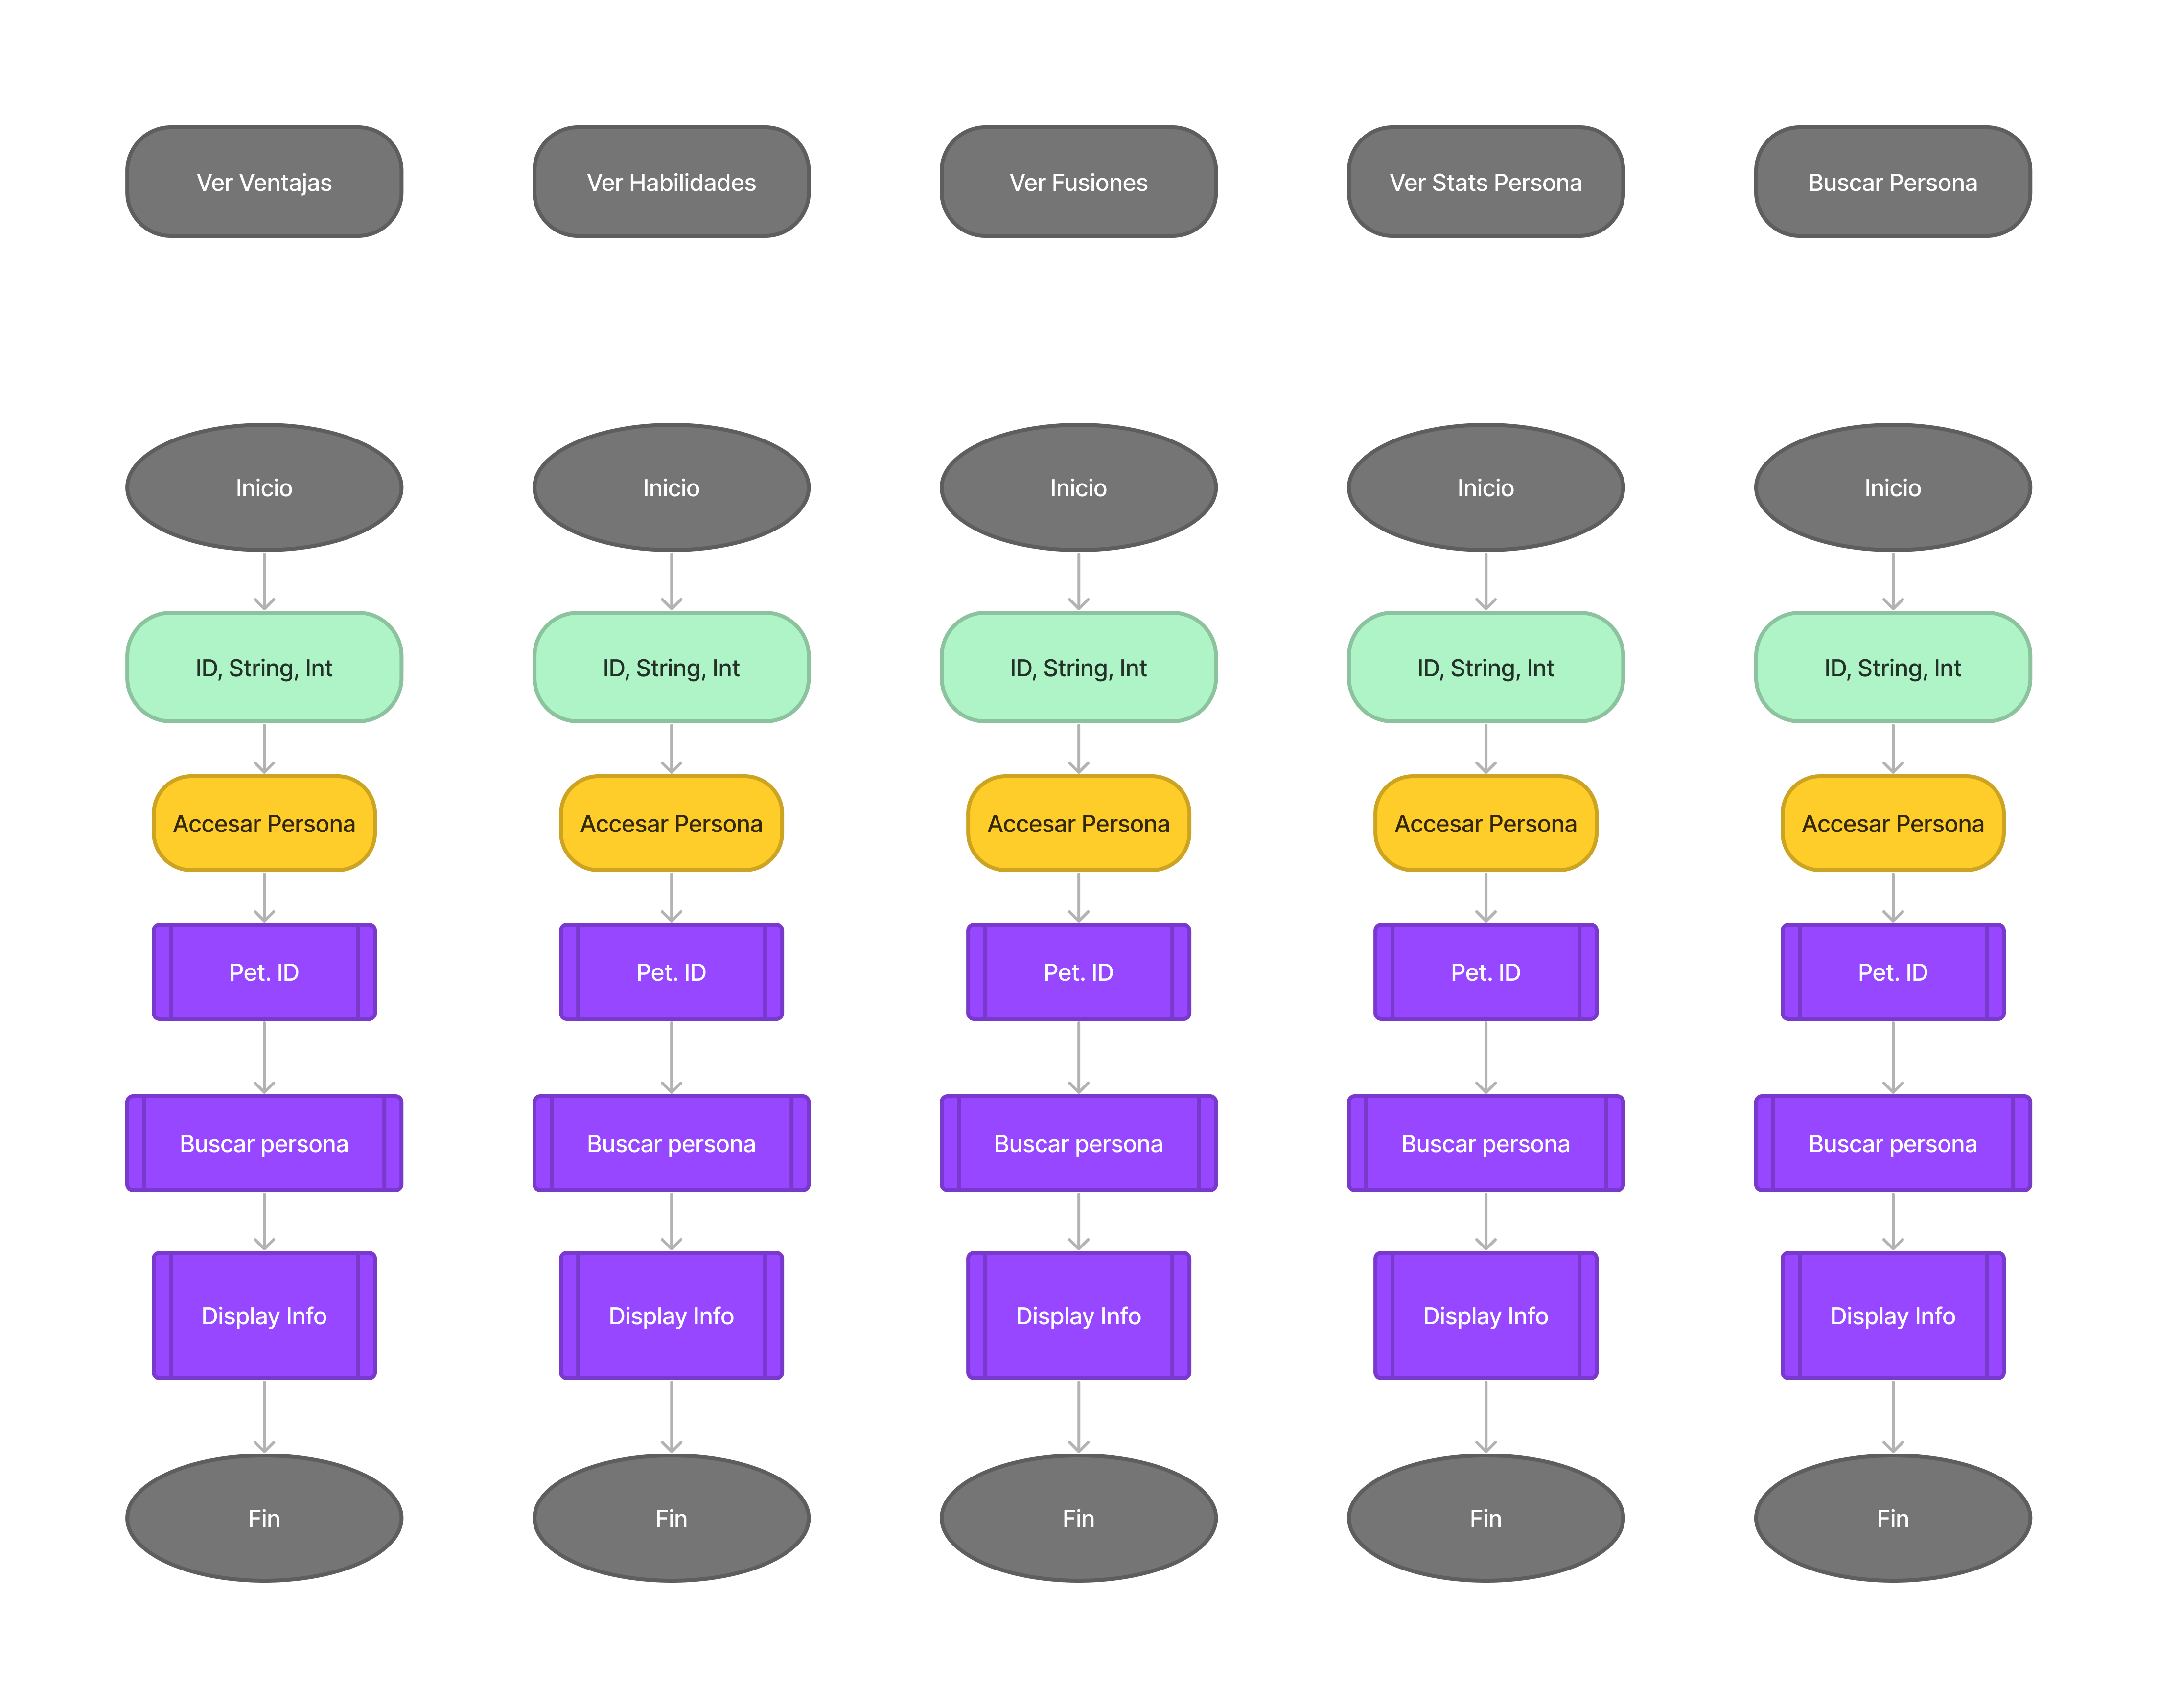
\includegraphics[width=1.0\textwidth]{DiagramaGaming3.png}

\section{Otro Diagrama de Clases}

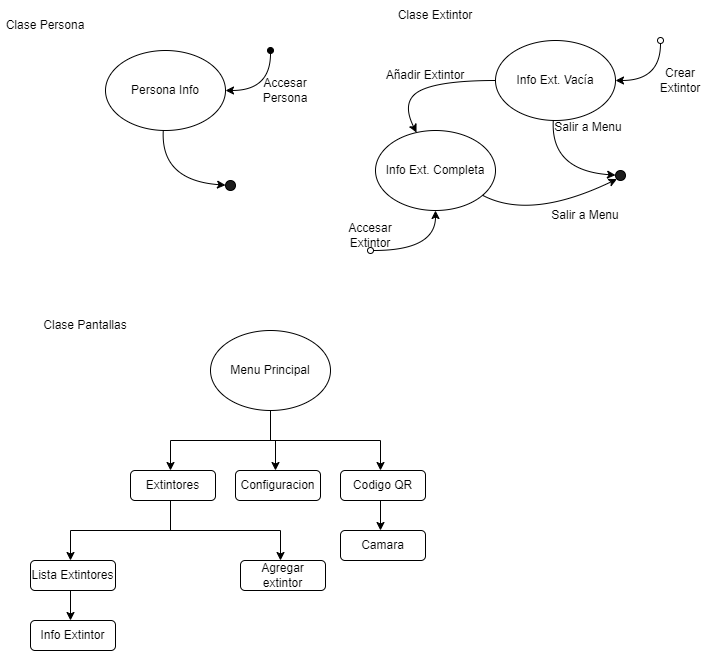
\includegraphics[width=1.0\textwidth]{El Gaming.png}

\newpage

\chapter{Links}

\href{https://www.figma.com/proto/lLCAXTlBZbxjpSGAWeCUPA/Skibidi-Gaming%7D?node-id=4-2&starting-point-node-id=4%3A2&mode=design&t=Sb1RTF0nqBBg2zxP-1}{Link a prototipado Figma Extintores}

\par .

\href{https://www.figma.com/proto/dMNLjaKBg1HFK16ZhoUZpI/Personongus?node-id=1-2&starting-point-node-id=1%3A2&mode=design&t=QmBVzDDLniVyYANz-1}{Link a prototipado Figma Persona 5}


\end{document}

